\section{Литературный обзор}

С целью поиска информации о локальном координационном числе (что в случае блужданий может также быть названо числом соседей узла), был проведён обзор литературы, возможно имеющей отношение к рассматриваемым в рамках проекта моделей.

\subsection{Livne, Meirovich: Polymers Adsorbed on a surface}

\subsubsection{Особенности модели блуждания}

В работе \cite{LivneSAW1988} исследуется поведение адсорбирующего случайного блуждания без самопересечений на кубической решётке со следующими особенностями симуляции

\begin{itemize}
    \item Случайное блуждание длины N+1  строится пошагово (N+1 мономеров в цепочке или N шагов), из начала координат (x=0, y=0, z=0) с ограничением на верхнее полупространство (то есть, z >= 0 и плоскость z=0 имеет открытые граничные условия).
    \item Энергия конформации считается как число мономеров, лежащих на поверхности (у которых $z_{i} = 0$), умноженное на константу взаимодействия полимера и поверхности $\epsilon$
    \item Вероятность i-й конформации считается последовательно: вводится новая статсумма, суммирующая для заданного направления текущей недостроенной цепочки всевозможные хвосты остаточной длины (10)\cite{LivneSAW1988}. 
\end{itemize}

\subsubsection{Подробнее о статсумме и методе Сканирования }

В данном подразделе вольным образом объясняется действие статсуммы, созданное методом сканированния. Так как при симуляции строится новое блуждание "c нуля", требуется оценка вероятности как каждого шага (точнее, направления $v_{k}$) так и всего блуждания.

Поэтому для k-го шага вероятность рассчитывается следующим образом:

\begin{enumerate}
    \item Считается статсумма куска будущего блуждания из b ($<= N - k + 1$) шагов, начинающая с направления v на высоте $z_{k-1}$:
    
    \begin{equation}
        Z_{k}(v, b, z_{k-1}, v_{k-1}) = \sum_{j}\exp{(-\epsilon m_{j}(0)/k_{b}T)}
        \label{Z_Lenvi}
    \end{equation}
     
    \item Затем проводится расчёт вероятности выбрать направление v из всех возможных на k-м шаге:
    
    \begin{equation}
        p_{k}(v|b,z_{k-1},v_{k-1}) = Z_{k}(v, b, z_{k-1}, v_{k-1}) / \sum_{v} Z_{k}(v, b, z_{k-1}, v_{k-1})
        \label{p_k_Lenvi}
    \end{equation}
    
    \item Итоговой вероятностью всего построения будет произведение всех вероятностей каждого шага по выбранным направлениям:
    
    \begin{equation}
        P_i(b) = \prod_{k=1}^{N} p_{k}(v_{k}|b,z_{k-1},v_{k-1})
    \end{equation}
\end{enumerate}

\subsubsection{Результаты работы}

Основными итогами работы являлось подтверждение эффективности метода "сканирования" для работы с длинными цепочками в модели адсорбирующего блуждания, определено критическое шкалирование перпердикулярного радиуса инерции (радиуса инерции проекции блуждания на ось z), а также профиля мономерной концентрации $p(z)$ (средняя доля узлов конформации длины N+1 на фиксированной высоте z от поверхности).

Информации о локальном координационном числе в статье найдено не было.

\newpage

\subsection{Madras, Sokal: The Pivot Algorithm}

Работа \cite{madras1988pivot} повествует о работе и эффективности алгоритма Пивота в изучении модели случайного блуждания без самопересечений (СБС).

\subsubsection{Основные принципы алгоритма}

Каждый шаг алгоритма проводит следующие действия над уже сгенерированной цепочкой длины N+1:

\begin{itemize}
    \item Случайно выбирается с равномерным распределением для рассматриваемых узлов $p_{k} = 1/N$ k-й узел цепочки ($0 <= k <= N-1$, хотя начальную точку k=0 на практике не используют)
    \item Последующую половину цепочки ($\omega_{k+1}, \omega_{k+2},\dots,\omega_{N}$ заменяют элементов группы симметрии (проще говоря, отражают, поворачивают или проводят комбинацию этих действий)
    \item В случае, если полученная операцией цепочка осталась без самопересечений, шаг принимается - в противном случае, шаг производится заново
\end{itemize}

В статье так же была доказана эргодичность алгоритма, а так же средние вероятности принятия каждого из возможных преобразований.

Для симуляций в качестве стартовой позиции использовалось два варианта: прямые цепочки ''rods'', при которых проволилось некоторое кол-во шагов до достижения термального равновесия системы (в таком состоянии процесс из следующих состояний цепочки становится близким по расспределению к стационарному стохастическому), или же ''димеризованные цепочки'' , состояние которых уже считается равновесным. Второй метод становится крайне времезатратным при большой длине цепочки, поэтому при N>=2400 чаще применялась термолизация прямых цепочек.

Пристальное внимание в статье было обращено к среднему радиусу инерции $S^{2}_{N}$ и квадрату расстояния между концами $\omega^{2}_{N}$, а так же к оценке метрической экспоненты $\upsilon$, характеризующей обе величины в крит. области модели: 

\begin{align*}
    \la \omega^{2}_{N} \ra &\sim N^{2\upsilon} \\
    \la S^{2}_{N} \ra &\sim N^{2\upsilon} 
\end{align*}

В оценке будущей работы было так же отмечено, что алгоритм Пивота не подходит для расчёта связующей $\mu$ и критической $\gamma$ экспонент (связующую константу так же называют \textit{эффективным координационным числом}), так как алгоритм алгоритм работает лишь в случае канонического ансамбля (при фиксированной длине цепочки) и требуется алгоритм, работающий уже в большом каноническом ансамбле (с цепочками изменяемой длины).

В статье не рассматривалось как таковое ''число соседей узлов''.


\subsection{Спицер, Основные принципы случайного блуждания, глава 3}

Данный подраздел посвящён рассмотрению случая двумерного возвратного случайного блуждания, движущемся по состояниям пространства $R$ (пространство целочисленных векторов размерности $d$) до достижения одного из элементов $A \subset R$. Под $T$ или $T_A$ мы будем подразумевать момент остановки - минимальное число $1<= k <= \infty$, такое что $x_k \in A$, то есть минимальное время достижение процессом {x_i} состояния из пространства A.

\subsubsection{Основные вероятностные функции}

Здесь будут более тщательно описаны используемые в главе функции вероятностей перехода.

Элементарной функцией, характеризующей случайное блуждание, является \textit{переходная функция $P(x,y)$}:

\[ 0 \leq P(x,y) = P(0, y-x) \]
\[ \sum_{x \in R} P(0,x) = 1 \]

Первое свойство крайне полезно в будущих рассуждениях, так как будет наследоваться многими следующими функциями и упрощает рассмотрение пространство
переходов до некоторой области вокруг начала координат. Например, в $G(x,y)$ - ожидаемое число попаданий в $y$ при начальной точке $x$:

\begin{equation}
G(x,y) = \sum_{n=0}^{\infty} P_n(x,y) = \sum_{n=0}^{\infty} P_n(0, y - x) = \sum_{n=0}^{\infty} P_x[x_n=y]
\end{equation}

$Q_n(x,y)$ определена на $(R-A) \times (R-A),\ \ n >= 0$ и обозначает вероятность попасть на n-м шаге попасть в $y$ (при $x_0 = x$), не попав за это время в A. Логично, что при остановке $T<n$ вероятность достижения на n-м шаге не существует, т.к. проццесс остановлен.

\begin{equation}
 Q_n(x,y) = P_x[x_n=y; T>n]
\end{equation}

Функция $H^{(n)}_A(x,y)$, наоборот, определяет вероятность n-м шаге остановиться в $y \in A$ (то есть, $y$ является первым состоянием из $A$, в которое попал процесс. В данном случае $H_A$ определено на $R \times A$

\begin{equation}
H^{(n)}_A(x,y) = 
	\begin{cases}
		P_x[x_T=y; T=n], \ \ \ x \in R-A \\
		0, \ \ \ x \in A, n>=1 \\
		\delta(x,y), \ \ \ x \in A, n=0
	\end{cases}
\end{equation}

$H_A(x,y)$ является обобщением предыдущей функции по времени, определяя лишь вероятность остановки процесса, начавшегося в $x$, в $y \in A$ и определена там же как и $H^{(n)}_A(x,y)$.

\begin{equation}
H_A(x,y) = 
	\begin{cases}
		P_x[x_T=y; T < \infty], \ \ \ x \in R-A \\
		\delta(x,y), \ \ \ x \in A
	\end{cases}
\end{equation}

Для случая $x \in R-A$ эту функцию можно определить так же как:

\begin{equation}
H_A(x,y) = \sum^{\infty}_{n=0}H^{(n)}_A(x,y)
\end{equation}

Особым случаем является вероятность $\Pi_A(x,y)$, существование которой обусловлено тем фактом, что время остановки должно быть натуральным числом - строго говоря, процесс может начатся в $x \in A$, пройти по ${x_1, x_2,...x_T-1 \in R-A}$ и остановиться в $y \in A$.

\begin{equation}
\Pi_{A}(x,y) = P_x[x_T=y, T < \infty]
\end{equation}

Последняя функция - $g_A(x,y)$, обобщает  по времени $Q_n$:

\begin{equation}
g_A(x,y) = 
	\begin{cases}
		\sum^{\infty}_{n=0}Q_n(x,y), \ \ \ x, y \in R-A \\
		0, otherwise
	\end{cases}
\end{equation}

\subsubsection{Соотношения между функциями}

Перейдём к некоторым предложениям из книги, которые позволят более полно понять природу некоторых функций в зависимости от начального состояния в них. Здесь будет описана лишь их вольная интерпретация, без доказательства.

Для произвольного случайного блуждания:

\begin{equation}
 \sum_{t \in R} P(x,t)H_A(t,y) - H_A(x,y) =  \begin{cases}
							\Pi_A(x,y)-\delta(x,y),\ \ \ x \in A, y\in A \\
							0,\ \ \ x \in R- A, y \in A
						        \end{cases}
	\caption{Предложение 10.1(а)}
\end{equation}

Пункт (а) предложения 10.1 проводит важную связь между $\Pi_A(x,y)$ и $H_A(x,y)$ при разных начальных состояниях: при $x \in R-A$ выражение равно нулю, как так оба слагаемых выражают один и тот же процесс из начального состояния до множества остановки, как со смещением (первое слагаемое), так и без него (правое). Равенство для случая $x \in A$ подтверждает раннюю интерпретацию функции $\Pi_A(x,y)$: шаг из множества остановки (P(x,t)) и затем движение из t до остановки снова в $A$.

\[ 0 \leq g_A(x,y) \leq g_A(y,y) \forall x, y \in R \]

То есть ожидаемое число попаданий из начального состояния x в y в обход A всегда меньше или равно чем ожидаемое число возвращений в начальное состояние. 
Если блуждание является апериодичным, то:

\[ g_A(x,x) < \infty \forall x \in R \]

Для $x \in R-A, y \in A$:

\[ H_A = \sum_{t \in R} g_A(x,t)P(t,y)\]

\[  G(x,y) = \sum_{t \in A} H_A(x,t)G(t,y) \]

\subsubsection{Начало потенциала}

Так как в движении блуждания важнейшую роль играет множество остановки (которое может быть как конечное, так и бесконечное), то основное внимание главы 
уделено распределению конечной точки блуждания $H_A(x,y), x \in R, y \in A$, обсуждение которого начинается с расширения предложения 10.1(а) (оно же 11.1):

\begin{equation}
 \sum_{t \in R} P_{n+1}(x,t)H_A(t,y) = H_A(x,y) + \sum_{t \in A} G_n(x,t)[\Pi_A(t,y)-\delta(t,y)], n \geq 0
\end{equation}

Необходимо заранее подчеркнуть, что это и последующие предложения считаются верными для апериодичных, возвратных, двумерных СБ. Примером такого служит простое
случайное блуждание на плоскости, которое исследовалось под названием Rand-Walk. 
Данное утверждение является первым шагом к исследованию распределения точки блуждания из бесконечно удаленной точки, однако перед этим выражение требует 
некоторых преобразований.

Крайне важным, хотя и очевидным утверждением является предложение 11.2:

\begin{equation}
 \sum_{t \in A} \Pi_A(t,y) = \sum_{t \in A} \Pi_A(y,t) = 1, \forall y \in A 
\end{equation}

Другими словами, апериодичные возвратные СБ рано или поздно при выходе из множества A попадут в него же. Теперь можно справедливо утверждать, что:

\[ \sum_{t \in A} \Pi_A(t,y) - 1 = \sum_{t \in A} [\Pi_A(t,y) - \delta(t,y)] = 0 \]

Следовательно, мы можем модифицировать 11.1 добавлением любой независимой от t константы, которая будет сокращаться при раскрытии суммы:

\begin{equation}
 \sum_{t \in R} P_{n+1}(x,t)H_A(t,y) = H_A(x,y) + \sum_{t \in A} [G_n(x,t) - G_n(0,0)][\Pi_A(t,y)-\delta(t,y)] = 
	H_A(x,y) - \sum_{t \in A} A_n(x,t)[\Pi_A(t,y)-\delta(t,y)] 
\label{eq:11_3}
\end{equation}

\[ A_n(x,y) = G_n(0,0) - G_n(x,y) = \sum_{k=0}^{n} [P_k(0,0) - P_k(x,y)]\]

Заметим, что A_n(x,y) так же наследует свойство пространственной однородности от G(x,y), которое получило его от P(x,y). Поэтому дальше мы частенько будем использовать слегка упрощенное определение этой функции - $a_n(x) = A_n(x,0)$

Именно начиная с утверждения \ref{eq:11_3} (формально, предложения 11.3) возникает задача перехода обоих частей предложения к пределу $n \to \infty$. Опуская доказательства существования пределов, положим следующие ответы.

\begin{enumerate}
\item $\lim_{n \to \infty} A_n(x,y)$ существует и определен как $A(x,y) = a(x-y)$ 
\item $\sum_{t \in R} P_{n+1}(x,t)H_A(t,y)$ существует, не зависит от t и определён как $\mu_A(y)$ 
\end{enumerate}

Пока что промежуточным после последних рассуждений выражением для распределения конечной точки СБ при бесконечном (или неопределенном) числе шагов является предложение 11.4:

\begin{equation}
 H_A(x,y) = \mu_A(y) + \sum_{t \in A} A(x,t)[\Pi_A(t,y)-\delta(t,y)]
 \label{eq:H_a_xy}
\end{equation}

Так же будет полезным рассмотреть не только движение из бесконечности до множества A, но и движение вокруг него - то есть, перемещение 
из $x \in A$ в $y \in A$. Очевидно, для этого важно более чётко определить способы использования функции $\Pi_A(x,y)$.

При рассмотрении некоторого конечного множества точек $B \subset R$, функция A(x,y) легко представима в виде матрицы ${A(x,y)}, x,y \in B$, которое называется 
\textit{сужением оператора $A(x,y)$ на $B$}. Такая матрица всегда имеет обратную, если $|B| \geq 2$ (предложение 11.8). Тем самым, мы получаем новый оператора
$K_B(x,y)$, определенный так же на $B \times B$:

\begin{equation}
 \sum_{t \in B} A(x,t) K_B(t,y) = \delta(x,y), x,y \in B
\label{eq:K_B} 
\end{equation}

Далее исследуемое остановочное множество мы будем обозначать как $B$, так как $A$ занято новой функцией.
Определим так же ещё несколько вспомогательных функций и константу:

\begin{align*} 
K_B(\cdot y) &= \sum_{x \in B} K_B(x,y)
K_B(x \cdot) &= \sum_{y \in B} K_B(x,y)
K_B(\cdot \cdot) &= \sum_{x \in B} \sum_{y \in B} K_B(x,y)
\end{align*}

Все эти инструменты помогут в определении и доказательстве основной теоремы параграфа, в которой, помимо самого предложения 11.4, есть нужная нам модификация.
В случае $x,y \in B$ для \ref{eq:H_a_xy} получим следующее выражение:

\[ \delta(x,y) = \mu_B(y) + \sum_{t \in B} A(x,t)[\Pi_B(t,y)-\delta(t,y)] \] 

Будет разумно перейти к матричной форме: левая часть будет единичной матрицей, первое слагаемое правой части будет матрицей $M_B$ размера $|B| \times |B|$, 
каждая строка которой - вектор значений \mu_B(y), а второе - результат произведения матрицами сужений оператора A(x,y) и $\Pi - E$ на $B \times B$. Получим:

\[ E = M_B + A \times (\Pi_B - E) \]

Применим оператор $K_B$ слева:

\[ K_B = K_B \times M_B + \Pi_B - E \]

Переход к элементам даст нам знакомые функции:

\[ K_B(x, y) = K_B(x \cdot) \mu_B(y) + (\Pi_B - \delta(x,y))\] 

Операция суммирования по строкам приведёт нас к двум важным пунктам теоремы:

\[ K_B(\cdot y) = K_B(\cdot \cdot) \mu_B(y) \rightarrow \mu_B(y) = \frac{K_B(\cdot y)}{K_B(\cdot \cdot)},\ \ \ K_B(\cdot \cdot) > 0 \]

Второй пункт выводится из ряда противоречий: если $K_B(\cdot \cdot) = 0$, то $K_B(\cdot y) = 0$ и матрица вырожденная и не имеет обратной (то есть, A(x,y) 
не существует). Если K_B(\cdot \cdot) < 0, то $K_B(\cdot y) < 0$, однако из определения K_B: 

\[ \sum_{t \in B} A(x,t) K_B(t,y) = \sum_{t \in B} K_B(x,t) A(t,y) = \delta(x,y) \rightarrow \sum_{t \in B} \sum_{x \in B} K_B(x,t) A(t,y) = 1 > 0 \]

$A(x,y) \geq 0$ из предложения 11.7, поэтому снова противоречие.
Подстановка первого доказанного пункта в ранние выкладки даст нам последний пункт теоремы:

\begin{equation}
\Pi_B(x,y) - \delta(x,y) = K_B(x,y) - \frac{K_B(x \cdot) K_B(\cdot y)}{K_B(\cdot \cdot)}
\label{eq:P_b}
\end{equation}

В итоге мы увидели, насколько мощным инструментом является функция $A(x,y)$ даже в сужении на $B$: её вычисление позволяет моментально рассчитать распределение 
конечного состояния из бесконечно удалённого, или распределение при возвращении во множество B. 
Ранние выкладки приводят к выводу, что $\mu_B(y)$ есть не что иное как вектор распределения вероятности остановиться в $y \in B$ из бесконечно удалённой точки.
Это будет доказано позже, однако мы уже сейчас и далее можем переопредлить эту переменную как $H_B{\infty, y}$. 
Теперь важнейшей задачей является расчёт самой функции $A(x,y)$, далее известное как ядро потенциала блуждания. 

\subsubsection{Основные вероятностные функции в СБ в контексте гармонического анализа}

Для начала необходимо определить основные понятия из теории гармонического анализа, которые понадобятся нам для вычисления ядра потенциала и его свойств.
Заранее определим два пространства: первое, это R как d-мерное пространство состояний блуждания $x = (x^1, x^2, x^3, \cdots, x^d)$, где $x^i$ - целые числа. 
Второе - это евклидово простанство $E$ такой же размерности: $\theta = (\theta^1, \theta^2, \theta^3, \cdots, \theta^d)$, где $\theta^i$ - вещественные числа.
К элементам обоих пространств применима операция модуля $|x|, |\theta|$, а между ними - скалярное произведение $x \cdot \theta$.

У блуждания действующем в пространстве $X$ c переходной функцией $P(x,y)$ существует \textit{характеристическая функция случайного блуждания}:

\[ \varphi(\theta) = \sum_{x \in R} P(0,x) e^{i x \cdot \theta}, \theta \in E \]

Основное действие, которое мы будет к ней применять и использовать для определения ранее известных функций, будет интеграл по кубу C (куб из пространства E 
с центром в начале координат и стороной $2\pi$):

\[ \int f d\theta = \int^\pi_\pi \cdots \int^\pi_\pi f(\theta) d\theta_1 \cdots d\theta_d \]

Теперь приведём некоторые примеры и увидим, насколько гармонический анализ упрощает работу с вероятностными функциями.

\[ (2\pi)^{-d} \int e^{i\theta \cdot (x-y)} d\theta = \delta(x,y) \]

Наконец, расширим соотношение характеристической и переходной функции для нескольких шагов блуждания:

\begin{align*}
\varphi^n(\theta) &= \sum_{x \in R} P_n(0,x) e^{i x \cdot \theta}
P_n(0,x) = (2\pi)^{-d} \int e^{i x\cdot \theta } \varphi^n(\theta) d\theta
\end{align*}

Теперь, мы можем возвращаться к определению a_n(x,y).

\[ a_n(x) = G_n(0,0) - G_n(x,0) = \sum_{k=0}^{n} P_k(0,0) - P_k(x,0) \]

Используя раннее определение k-й переходной функции через хар-ую функцию, получим:

\[ a_n(x) = (2\pi)^{-2} \int (1 - e^{i x\cdot \theta }) [1 + \varphi(\theta) + \cdots + \varphi^n(\theta)] d\theta = (2\pi)^{-2} \int \frac{1 - e^{i x\cdot \theta }}{1 - \varphi(\theta)} (1 - \varphi^{n+1}(\theta))d\theta

Опустим доказательство интегририруемости по Лебегу левой скобки итогового выражения и скажем лишь, что модуль правой скобки ограничен 2, а сама $\varphi^n(\theta)$ по определению по модулю меньше или равна 1 на всей области определения функции. Следовательно, в пределе $n \to \infty$ правая скобка сходится к единице и в итоге:

\[ a(x) = \lim_{n \to \infty} a_n(x) =  (2\pi)^{-2} \int \frac{1 - e^{i x\cdot \theta }}{1 - \varphi(\theta)}d\theta \]

Итак, весь аппарат исследования поведения блуждания в пространстве с остановочным множеством готов к использованию. Однако полученная формула кажется несколько
неудобной - придётся считать потенциал в каждой исследуемой точки, вблизи она или далеко от начала координат. Следующий подраздел поможет справиться с данной преградой.

\subsubsection{Блуждание с бесконечно удалённой начальной точкой}

Данный раздел посвящён асимптотическому поведению ядра потенциала блуждания $A(x,y)$, начальная точка бесконечно удалена от начала координат (случай $|x| \to \infty$).
Первый момент - это утверждение 12.2:

\[\lim_{|x| \to \infty}[A(x, y_1) - A(x, y_2)] = 0 \]

Утверждение будет более применимо в контексте $a(x)$ - тогда мы говорим не о разнице между значениями ядер потенциалов с разными конечными точками, а
о разнице между значениями ядер потенциалов с двумя бесконечно удалёнными точками, тем самым обобщая это определение на расстояние нач. точки от начала координат:

\[\lim_{|x| \to \infty}[a(x + y) - a(x)] = 0 \]

Далее вычислим саму асимптотическую функцию для $a(x)$. 
Для упрощения ведения записей мы продолжим говорить только о простом случайном двумерном блуждании:

\[ \lim_{|x| \to \infty}[a(x) - \frac{2}{\pi}\ln{|x|}] = \frac{1}{\pi}\ln{8} + \frac{2\gamma}{\pi} \]

где $\gamma = 0.5572\cdots$ - постоянная Эйлера.

Последнее незаписанное свойство ядра $A(x,y) = a(x-y)$, которое понадобится нам на практике и будет полезно для расчётов значений потенциалов рекурсивным 
методом - это следующее равенство, доказываемое ровно из определения:

\begin{equation}
 \sum_{y \in R} P(x,y)a(y) - a(x) = \delta(x,0) 
 \label{eq:13_3}
\end{equation}

Оно будет отправной точкой для расчётов потенциала, начиная из начала координат, как будет видно в следующем разделе. 

\subsubsection{Расчёт потенциала на практике для Rand_Walk}

Начнём с небольшого преобразования интегральной формулы ядра потенциала:

\[ a(x) = (2\pi)^{-2} \int \frac{1 - e^{i x\cdot \theta }}{1 - \varphi(\theta)}d\theta = (2\pi)^{-2} \left[\int \frac{1 - \cos{x\cdot \theta}}{1 - \varphi(\theta)}d\theta - i\int \frac{\sin{x\cdot \theta}}{1 - \varphi(\theta)}d\theta\right]\]
\[ \varphi(\theta) = \frac{1}{4} [e^{i\theta_1} + e^{i\theta_2} + e^{-i\theta_1} + e^{-i\theta_2}] = \frac{1}{2} [\cos{\theta_1} + \cos{\theta_2}]\]

Ввиду симметричности области интегрирования, правый интеграл обращается в ноль. Более того, в купе с четностью косинуса в левой слагаемом, получим:

\[ a(z) = a(-z) = a( \bar z) = a(- \bar z) = a(i z) = a( -iz)\]

Здесь нужно подчеркнуть, что мы всё так же работаем с векторами с целочисленными коэффициентами. 
Просто для более короткой записи мы сопоставляем каждому вектору $x = (x_1, x_2)$ комплексное число $z = x_1 + i x_2$, которое и записываем в качестве аргумента a(x).
Полученное свойство обозначает симметрию значений потенциала по обоим осям плоскости, а так же относительно обоих диагоналей. 
Это позволяет рассчитывать лишь одну восьмую всей оси.

Пользуясь свойством симметрии в выражении \ref{eq:13_3} в случае x = 0, при том что a(0) = 0, получим, что $a(1) = a(-1) = a(i) = a(-i) = 1$.
Нетронутыми остались значения на диагоналях, которые придётся честно считать через интеграл, однако полную выкладку мы опустим:

\begin{equation}
 a(n + i n) = \frac{4}{\pi} \sum_{k=1}^{n} \frac{1}{2k-1} 
 \label{eq:diag_a}
\end{equation}

Рассчёт остальных точек будет протекать через уравнение \ref{eq:13_3}, где неизвестная переменная является одной из соседних по отношению к известной.
Вычисление ряда будет начинаться от точки на оси к диагонали.

\subsubsection{Решение задачи}

Собрав вместе \ref{eq:H_a_xy}, \ref{eq:P_b} и методы расчёта потенциала для любой точки, перейдём непосредственно к исследумой задаче соседей (III.9).
Чтобы регистрировать не только попадания блуждания в начало координат, что будет означать ''полную остановку'' блуждания, определим все пять точек ($z = \{ -1, 0, 1, i, -i \}$) как остановочное множество B. 
Учитывая, с какими сложными вероятностными функциями мы можем теперь работать, идейно задача упрощается до случайного процесса, состояния в котором - те самые соседние к началу координат точки.
Тогда вероятностью перехода между той или иной точкой будет выступать $\Pi_B(x,y)$ - её результат не зависит от времени (числа шагов, проведённых между точками множества B $n$).
Более того, построенное такими образом множество B ограничивает способы попасть из одной гран. точки в другую - $x = 0 \in B$ требует проходить между гран. точками только ''вокруг'' $B$. 

Первым пунктом решения задачи рассчитаем матрицу сужения оператора $A(x,y) = a(x-y)$ на множество $B$.
Ввиду сильного свойства симметрии функции $a(x)$ и минимального разброса между точками $B$, достаточно рассчитать следующие потенциалы:

\begin{itemize}
\item $a(1) = 1$ - для всех пар $A(x,0)$ и $A(0,y)$, $x, y \neq 0$, так как краевые точки по условию задачи - соседние к началу координат
\item $a(1+i) = \frac{4}{\pi} \eqref{eq:diag:a}$ - для пар смежных крайних точек (например, $\pm i$ и $ \pm 1$)
\item $a(2) = 4 - \frac{8}{\pi}$ - между парами противолежащих точек ($A(1,-1), $A(i,-i)$)  
\end{itemize} 

Последний потенциал легко считается из уравнения \eqref{eq:13_3} в случае $x = 1$.
Полученная матрица сужения оператора имеет вид:

\begin{equation}
A_B(z_i, z_j) = 
	\begin{pmatrix}
		0 & 1 & 4 - \frac{8}{\pi} & \frac{4}{\pi} & \frac{4}{\pi} \\
		1 & 0 & 1 & 1 & 1 \\
		4 - \frac{8}{\pi} & 1 & 0 & \frac{4}{\pi} & \frac{4}{\pi}\\
		\frac{4}{\pi} & 1 & \frac{4}{\pi} & 0 & 4 - \frac{8}{\pi}\\
		\frac{4}{\pi} & 1 & \frac{4}{\pi} & 4 - \frac{8}{\pi} & 0 \\
	\end{pmatrix}
\end{equation}
\[ z = \{ -1, 0, 1, i, -i \} \]

Далее рассчитаем матрицу $K_B$ \eqref{eq:K_B}, которая является обратной к $A_B$:

\begin{equation}
K_B = 
	\begin{pmatrix}
		-0.573 & 0.25 & 0.115 & 0.229 & 0.229 \\
		0.25 & -1 & 0.25 & 0.25 & 0.25\\
		0.115 & 0.25 & -0.573 & 0.229 &  0.229\\
		0.229 & 0.25 & 0.229 & -0.573 & 0.115\\
		0.229 & 0.25 & 0.229 & 0.115 & -0.573\\
	\end{pmatrix}
\end{equation}

\[ K_B( \cdot y) = \{ 0.25, 0, 0.25, 0.25, 0.25\},\ \ \ \ \ K_B(\cdot \cdot) = 1 \rightarrow H(\infty, y) = \{ 0.25, 0, 0.25, 0.25, 0.25\}\]

Сейчас мы получили распределение начальной остановочной точки блуждания - первая точка из множества $B$, в которую попадёт блуждание - из бесконечно удалённой точки.
Очевидно, второе значение вектора вероятностей, соответствующее началу координат ($z = 0$) равно нулю, в него невозможно попасть никак иначе, чем через соседние состояния.
Вероятности попасть в них, в свою очередь, распределены равномерно - это объясняется тем, что при протекании блуждания из бесконечности, оно с большой вероятностью несколько раз обойдёт множество $B$.
Тем самым, блуждание ''забывает'' свои предыдущие состояния и следовательно, направление.

Последним вычислительным пунктом задачи будет подсчёт матрицы $\Pi_B$ по формуле \eqref{eq:P_b}:

\[ \Pi_B(x,y) = K_B(x,y) - \frac{K_B(x \cdot) K_B(\cdot y)}{K_B(\cdot \cdot)} + \delta(x,y) \]

В матричном виде это примет вид:

\[ \Pi_B = (K_B)_{|B| \times |B|} - K_B(x \cdot)_{|B| \times 1} \times K_B(\cdot y)_{1 \times |B|} / K_B(\cdot \cdot) + E_{|B| \times |B|}

\begin{equation}
\Pi_B = 
	\begin{pmatrix}
		0.365 & 0.25 & 0.053 & 0.166 & 0.166 \\
		0.25 & 0 & 0.25 & 0.25 & 0.25\\
		0.053 & 0.25 & 0.365 & 0.166 &  0.166\\
		0.166 & 0.25 & 0.166 & 0.365 & 0.053\\
		0.166 & 0.25 & 0.166 & 0.053 & 0.365\\
	\end{pmatrix}
\end{equation}

Получение данной матрицы имеет огромное значение, т.к. любой выход из множества $B$ и возвращение обратно будет оцениваться именно через эту матрицу.
Мы точно знаем, что для двумерных возвратных апериодичных блужданий возвращение в $B$ при выходе из него гарантирован, поэтому все движения вне множества ''сжимаются'' до единовременного
перехода между ними.
В итоге, как было сказано ранее, задача о случайном блуждании и соседних началу координат состояниях упрощена до задачи случайного процесса с матрицей перехода $P_B$ и начальным распределением $H(\infty,y)$:
теперь количество посещенных соседних началу координат точек интерпретируется как количество посещённых уникальных состояний до первого достижения состояния 2 (z=0).
Последовательность точек блуждания $\{X_i\} \subset R$ так же теперь упрощена до последовательности ''остановок'' $\{Z_{i^*}\} \subset B$. Обе последовательности заканчиваются точкой $x_T = z_{T^*} = 0$.

Перейдём непосредственно к расчёту вероятностей блуждания из бесконечно удалённой начальной точки посетить фиксированное число соседей.
В первую очередь рассчитаем вероятность, что блуждание посетит лишь одну соседнюю точку $\lim_{|x| \to \infty} P_x[N=1] = p_1$. 
Из определения простого случайного блуждания количество попаданий в одну и ту же соседнюю точку не ограничивается.
Поэтому блуждания класса $P_1$ имеют вид $\{X_i\}_{p1} = \{c, c, \cdots, c, 0\}, c=const$.
Формула вероятности таких блужданий имеет следующий вид:

\begin{align*}
P_1 &= \sum_{t \in \{1, -1, i, -i\}} H(\infty, t) (P_B(t, 0) + P_B(t,t) (P_B(t,0) + P_B(t,t) (\cdots)) = \\
    &= \sum_{t \in \{1, -1, i, -i\}} H(\infty, t) P_B(t,0) (1 + P_B(t,t) + P_B^2(t,t) + \cdots + P_B^2(t,t) + \cdots) = \\
    &= \sum_{t \in \{1, -1, i, -i\}} 0.25 \times 0.25 \sum_{k=0}^{\infty} P_B^k(t,t)
\end{align*}

\[ P_B(t,t) = 0.365\ \ \  \forall t \in B \rightarrow P_1 = 0.25 \sum_{k=0}^{\infty} 0.365^k = \frac{0.25}{1 - 0.365} = 0.3936 \]

Следующей ступенью решения задачи будет расчёт $P_2$.
Здесь задача усложняется тремя разными случаями - в зависимости от того, как блуждание перемещается:

\begin{enumerate}
\item между первой точкой остановки $z_0$ и правой смежной точкой (идущая по часовой стрелке)
\item между $z_0$ и левой смежной точкой
\item между $z_0$ и противоположной ему точкой
\end{enumerate}

Вероятности перейти к левой смежной точке и правой смежной точке равны $0.166$, к противоположной - $0.053$.
Назовём эти вероятности перехода на каждой шаге $p_t, p_o$ (''probability of the turn'', ''probability of the opposite'').
Вероятность вернуться в то же граничное состояние равно $0.365$ для любой точки.
Эту вероятность определим как $p_{t0}$.
Вероятность перейти в конечное состояние $z_T = 0$ тоже независима и будет определена как $p_e$ (Probability of the End).
Тогда вероятность ''блуждание пройдёт хотя бы по одной из двух точек'' $P_2^*$ имеет следующий вид:

\begin{align*)
P_2^* &= 2 * \sum_{t \in \{1, -1, i, -i\}} H(\infty, t) (p_e + (p_t + p_{t0}) (p_e + (p_t + p_{t0}) (\cdots)) + 
      &+ \sum_{t \in \{1, -1, i, -i\}} H(\infty, t) (p_e + (p_o + p_{t0}) (p_e + (p_o + p_{t0}) (\cdots))
\end{align*}

Первое слагаемое удвоенно, так как здесь подсчитываются вероятности передвижения между начальной и смежной левой и между начальной и смежной правой.
Вторая сумма - это вероятность передвижения между начальной и противоположной точкой.

Во всех случаях идёт суммирование по всем начальным точкам, что может вызвать сомнение - кажется, что мы подсчитываем одну блуждание между одной пары точек два раза.
Однако если представить блуждание как последовательность $\{Z_i\} \subset B$, то единственное состояние, которое не регулируется скобкой - начальное. 
Поэтому подсчёт проходит для каждого возможного начального состояния.

Ранее было уточнено, что результатом расчёта является ''вероятность'' что блуждание посетит хотя бы одну точку из двух - 
ещё не гарантируется, что блуждание посетит обе точки за всё время. 
Более того, очевидно, что мы несколько раз приблавляем вероятность что блуждание посетит одну точку (по одному на каждый подсчёт блуждания с фиксированным нач. состоянием, то есть, три).
Тогда чтобы ''запретить блужданию'' достигать начала координат через лишь одну точку, необходимо три раза вычесть $P_1$:

\[ P_2 = P_2^* - 3 P_1 = 1.4957 - 3 * 0.3937 = 0.3146 \]

Последним этапом будет рассчёт $P_3$ (так как очевидно, что $P_4 = 1 - P_1 - P_2 - P_3$). 
Данный случай значительно сложнее предыдущих: если зафиксировать тройку соседей $z_{i1}, z_{i2}, z_{i3}$, между который блуждание перемещается до достижения начала координат (назовём их ''разрешёнными соседями''),
то возникает серьёзная проблема рассчёта вероятности на каждом шаге - если текущая точка блуждания лежит в центре разрешенной тройки (то есть, обе смежные текущей точки являются так же разрешёнными),
то вероятность остаться в этой тройке равна $0.365 + 2 * 0.166 = 0.697$. Если же текущая точка - крайняя по отношению к разрешённой тройке, то вероятность ниже - $0.365 + 0.166 + 0.053 = 0.584$, поскольку одна из 
разрешённых точек находится на протиположной стороне множества $B$.

Получается, нужная нам вероятность остаться в ''разрешенном подмножестве'' не постоянная, а зависит от предыдущего состояния процесса $\{Z_i\}$.
Значит, решить эту подзадачу по способу расчёта предыдущих вероятностей уже не получится.
Подойдём к ней со стороны её матрицы перехода. Очевидно, что любой последовательности $\{Z_i\} = \{z_0, z_1, \cdot, z_{T^*} = 0\}$ можно поставить в соответствие её вероятность:

\[ P = H(\infty, z_0) P_B(z_0, z_1) \cdots P_B(z_{T^*-1}, 0) \]

Выходит, что вероятности блужданий, ни разу не посетившие одну фиксированную точку $\hat z$ (назовём её ''запрещённой''), не имеют в своей записи $P_B(\ , \hat z), P_B(\hat z,\ )$ и $H_B(\infty, \hat z)$.
Эта идея позволяет нам использовать для расчёта модифицированные матрицы переходной функции $P_B[\hat z](x,y)$, такие, что $P_B(\ , \hat z) = 0$ и $P_B(\hat z,\ ) = 0$ - то есть,
строки и столбцы запрещённого состояния просто занулены. То же самое мы делаем и с начальным распределением - определим $H_B [\hat z]$, такое что $H_B(\infty, \hat z) = 0$.
Так же, по условию, что блуждание останавливается в точке начала координат, мы можем объявить состояние $z=0$ поглощающим, то есть - занулить вероятности выхода из состояния 0 в любые другие, а вероятность P_B(0,0) объявить равной 1.

Тогда вероятность $P_3$ расчитывается следующим образом в матричном виде:

\begin{equation}
P_3 = \sum_{t \in \{1, -1, i,  -i\}} \lim_{k \to \infty} H_B[t] P_B^k[t] - 3 P_1 - 2 P_2
\end{equation}

Поскольку первое слагаемое подсчитывает блуждания которым ''запрещено'' посещать одну и из точек, мы никак не ограничиваем посещения лишь одной или двух из трёх разрешённых точек.
$P_1$ вычитается трижды (за каждый раз, когда фиксированная точка становится разрешенной), $P_2$ - дважды (за каждый раз, когда фиксированная пара остается разрешенной).

Заметим так же, результатом выражения под знаком суммы будет сумма вероятностей всех блужданий, прошедших по любым точкам кроме t (так как вероятность иного блуждания содержит хотя бы один нулевой множитель).
В качестве наглядного примера рассчитаем одно из слагаемых - $\lim_{k \to \infty} H_B[i] P_B^k[i]$. По определению: 
\[ H_B[i] = \{0.25, 0, 0.25, 0, 0.25\} \]
\begin{equation*}
 P_B[i] = 
 \begin{pmatrix}
	0.365 & 0.25 & 0.053 & 0 & 0.166 \\
	0 & 1 & 0 & 0 & 0 \\
	0.053 & 0.25 & 0.365 & 0 &  0.166 \\
	0 & 0 & 0 & 0 & 0 \\
	0.166 & 0.25 & 0.166 & 0 & 0.365\\
 \end{pmatrix} 
\end{equation*}

Найдём собственные значения и вектора матрицы P_B[i]:

\begin{equation*}
 P_B[i] = S\times D \times S^{-1}, \\
 D = Diag(0.6277, 0.312, 0.1546, 1, 0) \\
 S = 
 \begin{pmatrix}
	-0.527 & -0.707 & 0.471 & 0.416 & 0 \\
	0 & 0 & 0 & 0 & 0.654 \\
	-0.527 & -0.707 & 0.471 & 0.416 & 0 \\
	0 & 0 & 0 & 0 & 1.0 \\
	-0.666 & 0 & -0.745 & 0.475 & 0 \\
 \end{pmatrix} 
\end{equation*}

Такое разложение позволяет нам получить следующий предел:
\begin{equation*}\lim_{k \to \infty} P_B[i]^k = lim_{k \to \infty} (S\times D \times S^{-1})^k = S \times lim_{k \to \infty} D^k \times S^{-1} \end{equation*}
\begin{equation*}\lim_{k \to \infty} D^k = lim_{k \to \infty} Diag (0.6277^k, 0.312^k, 0.1546^k, 1^k, 0^k) = Diag(0,0,0,1,0) \end{equation*}


В конечном счёте:

\begin{equation*}
	\lim_{k \to \infty} H_B[i] P_B^k[i] = H_B[i] (S \times Diag(0,0,0,1,0) \times S^{-1}) = \{0.25, 0, 0.25, 0, 0.25\} \times 
	\begin{pmatrix}
	0 & 0.6366 & 0 & 0 & 0 \\
	0 & 0 & 0 & 0 & 0 \\
	0 & 1. & 0 & 0 & 0 \\
	0 & 0.6366 & 0 & 0 & 0 \\
	0 & 0.7268 & 0 &0 & 0 \\
	\end{pmatrix} 
	= 0.5
\end{equation*}

Из геометрической симметрии множества $B$ и симметрии её нормальной матрицы перехода следует, что при запрете любой точки можно переставить состояния
в матрице так, чтобы получить такую же матрицу $P_B[\hat z]$, как раньше. Поэтому:

\begin{equation}
P_3 = \sum_{t \in {1, -1, i,  -i}} 0.5 - 3 P_1 - 2 P_2 = 0.19
\end{equation}

И наконец, завершающая подзадача:

\begin{equation}
P_4 = 1 - P_1 - P_2 - P_3 = 0.1018
\end{equation}

\subsubsection{Сравнение результатов с прямой задачной симуляцией}

Результаты расчётов совпадают с подсказкой из задачи - действительно, пусть они не идеально точно, но $P_1:P_2:P_3:P_4 \approx 4:3:2:1$.
 
Так же результаты были проверены симуляцией Монте-Карло - за основу бралась упрощённая модель случайного процесса с матрицей перехода $P_B$ и
начальным распределением $H_B(\infty, y)$. 

\begin{figure}
    \centering
    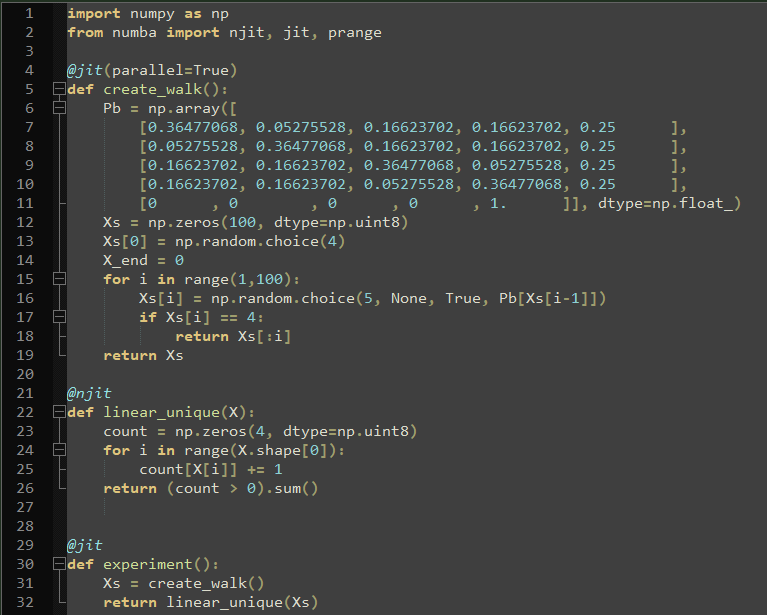
\includegraphics[width=0.8\textwidth]{Sections/Images_2/code_1.png}
    \caption{Исполнительная часть симулирующего кода, подсчитывающая кол-во посещённых точек до достижения начала координат}
    \label{fig:lattices}
\end{figure}

Процесс симулировался до достижения состояния $z=0$ или до длины 100 (так как вероятность, что за такое время процесс ни разу не пройдёт
это состояние пренебрежимо мала $\approx 3 * 10^{-13}$).

\begin{table}[h!]
    \centering
    \begin{tabular}{|c|c|c|c|c|}
        \hline
        P_1 & P_2 & P_3 & P_4 & steps \\ \hline
         0.393539 & 0.314722 & 0.190020 & 0.101719 & 226020000 \\ \hline
		 0.393567 & 0.314689 & 0.190020 & 0.101725 & 449140000 \\ \hline
		 0.393566 & 0.314680 & 0.190025 & 0.101729 & 638220000 \\ \hline
    \end{tabular}
    \caption{Доли блужданий, прошедших 1-4 уникальных состояний до достижения начала координат - и количество симулированных блужданий}
    \label{tab:spitser_res_simple}
\end{table}

Из таблицы \ref{tab:spitser_res_simple} видно, что результаты совпадают с рассчитанными вероятностями.

Была так же попытка сделать модель случайного блуждания, идущего из точки на расстоянии R от начала координат, однако доля блужданий, 
которые не смогли добраться до начала координат за $R * 10^6$ была огромна. Поэтому ''полный'' вариант симуляций был упрощён.

\begin{table}[h!]
    \centering
    \begin{tabular}{|c|c|c|}
        \hline
        R & P_{error} & steps \\ \hline
        10 & 0.413071 & 70000  \\ \hline
		20 & 0.477033 & 30000 \\ \hline
		50 & 0.533500 & 10000  \\ \hline
    \end{tabular}
    \caption{Доли блужданий с начальной точкой на расстоянии R, не достигших начала координат за $R * 10^6$ шагов - и количество симулированных блужданий}
    \label{tab:spitser_res_full}
\end{table}


\subsubsection{Сравнение результатов с симуляцией Rand-Walk}

Ранее в рамках проекта 19455 ''Решеточные модели макромолекул'' была проведена генерация модели случайного блуждания с самопересечениями 
(далее Random-Walk) для фиксированных длин $10^{2}-10^{4}$. 
Рассматривалась доля узлов с фиксированным числом соседей - от 1 до 4 - среди уникальных узлов в итоговой конформации, для чистоты результатов и 
возможности сравнения с результатами случайного блуждания без самопересечений. Доли уникальных узлов так же бралась во внимание при симуляциях. 
Результаты симуляций, а так же количество итераций для каждой длины, описаны в таблице \ref{tab:Ran_Walk_neigh} и изображены на графике \ref{fig:Rand_Path_N1_4}

\begin{table}[h]
    \centering
    \begin{tabular}{|c|c|c|c|c|c|c|}
        \hline
        N & $steps$ & $unique$ & $n_{1}$ & $n_{2}$ & $n_{3}$ & $n_{4}$ \\ \hline
        100 & 7450000 & 0.49(8) & 0.07(3) & 0.33(9) & 0.36(7) & 0.24(9) \\ \hline
        200 & 5684000 & 0.44(7) & 0.05(2) & 0.29(7) & 0.35(5) & 0.30(9) \\ \hline
        500 & 2045000 & 0.39(6) & 0.04(1) & 0.24(5) & 0.34(4) & 0.38(8) \\ \hline
        1000 & 654000 & 0.36(5) & 0.03(1) & 0.22(4) & 0.33(4) & 0.42(7) \\ \hline
        2500 & 132000 & 0.33(4) & 0.027(7) & 0.19(3) & 0.31(3) & 0.48(6)  \\ \hline
        5000 & 37000 & 0.31(4) & 0.024(5) & 0.17(3) & 0.29(3) & 0.51(6) \\ \hline
        10000 & 10000 & 0.29(3) & 0.021(4) & 0.16(2) & 0.28(3) & 0.54(5) \\ \hline
    \end{tabular}
    \caption{Средние доли узлов c 1-4-мя соседями в конформациях модели Random-Walk длин $10^{2}-10^{4}$}
    \label{tab:Ran_Walk_neigh}
\end{table}

\begin{figure}[]
    \centering
    \caption{Зависимость долей узлов с фиксированным число соседей в случайном блуждании от обратного кол-ва шагов в конформации 1/N}
    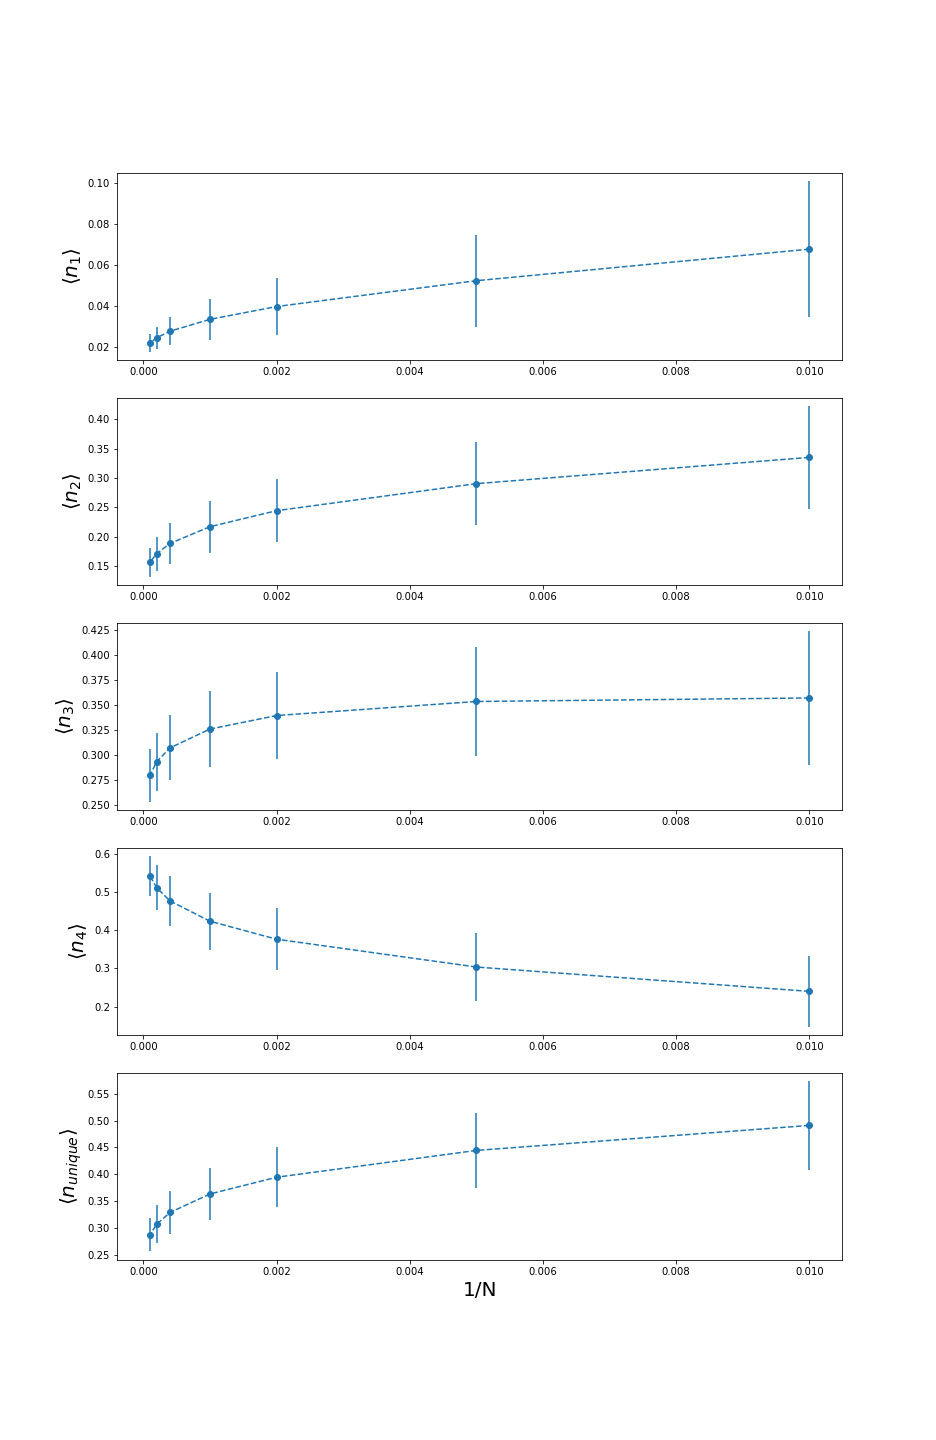
\includegraphics[width=0.9\textwidth]{Sections/Images/Rand_Path_N1-4_unique.png}
    \label{fig:Rand_Path_N1_4}
\end{figure}

На таблице видно явное несовпадение значений $n_{i}$ из исследований Rand-Walk фиксированной длины и $P_i$ из задачи Спитцера. 
Оно может быть объяснено следующим образом:

Можно сказать, что обе задачи являются обращениями друг друга - начало координат в Rand-Walk фикс. длины является начальной точкой блуждания, 
в то время как в задаче Спитцера - конечной. Это имеет принципиальную разницу, так как в первом случае начало координат может быть посещено бесконечное
количество раз, что позволяется быстро перемещаться между его соседними блужданиями, а в другом - лишь однажды.

На основании полученных результатов можно сделать вывод, что при условии бесконечного количества шагов результаты обоих задач показавают поведение разных
аспектов простого случайного блуждания.



